\section{Deep Reinforcement Learning}

"Playing Atari with Deep Reinforcement Learning" \cite{mnih2013playing} and "Deep Reinforcement Learning: Pong from Pixels" \cite{karpathy2016deep} show how applying Deep Reinforcement Learning for the game of pong leads to the best results.\\

The policy function, or policy network, used to decide what to do based on the current state, is a fully connected neural network with n hidden layers, which is why this method is called Deep RL. In the papers frame image of the game is taken as input, in which each pixel corresponds to a single input neuron, and returns a number between 0 and 1 which can be seen as the probability to win with a given action (e.g. left). If the number is greater than 0.5 we go to the left, otherwise we go to the right. If it is 0.5, a random choice is made. To do this, the output neuron has a sigmoid function \cite{mnih2013playing}\cite{karpathy2016deep}.
Since politics generates probability, this politics is stochastic.

\begin{figure}[ht]
    \centering
    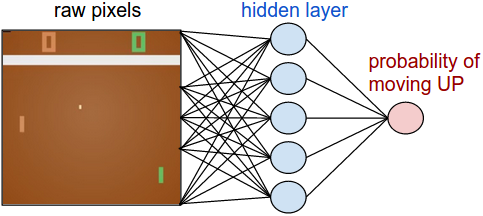
\includegraphics[scale=0.4]{images/DRL_network.png}
    \caption{Simple image of the policy network of an Deep RL system.}
    \label{fig:DRL_network}
\end{figure}

This can also be easily applied to inputs of a different nature, such as vectors representing the position of the ball, the direction, the position of the paddles, etc. \\

A very big advantage that Deep RL offers is that it can handle unseen states well \cite{mnih2013playing}\cite{karpathy2016deep}. This is because a large portion of pixels could be similar to an image already seen and on which the NN has been trained, so the network is likely to produce a similar prediction to the image seen previously. Instead, algorithms like MDP behave randomly in these cases. \\

Generally, to facilitate learning, pre-processing is applied.
An image can then be cropped to eliminate those pixels that are not needed for prediction, such as the scoreboard. Other things that can help are grayscaling the image and reducing image resolution \cite{mnih2013playing}.

\subsection{Deep Q Network}
Deep Q Networks(DQN) were introduced in "Playing Atari with Deep Reinforcement Learning" \cite{mnih2013playing}.
A DQN is a CNN adapted for RL used as a function approximator to estimate the Q-values, where the inputs are images and the outputs depends on the task's number of actions.
The loss is defined as the mean squared error between the Q-value target and the network's predicted at step $i$.

$L(\theta_i) \leftarrow \mathbb{E}_{s, a, r, s'} [((r + \gamma \max_{a'} Q(s', a'; \theta_i)) - Q(s, a; \theta_{i-1}))^2]$
where s is the current state, s' the next state, a the current action selected by the $\epsilon$-greedy policy, r the immediate reward and $\theta$ are the network parameters.

To avoid computing the full expectation in the DQN loss, we can minimize it using stochastic gradient descent

Experience Replay is a technique introduced in The Atari DQN work to make the network updates more stable.
This method At each time step of data collection, add the transitions to a circular buffer called the replay buffer.

Given a random batch of transitions $(s, a, r, s')$ from the replay buffer we can calculate the loss at step $i$ as the following formula
$L(\theta_i) \leftarrow ((r + \gamma \max_{a'} Q(s', a'; \theta_i)) - Q(s, a; \theta_{i-1}))^2$

Better describe the stability problem of DQN... Non-stationary or unstable target
